\documentclass[logo,reportComp]{thesis}
\usepackage[cpp,linenum]{mypackage}

\title{计算机图形学}
\subtitle{作业四:贝塞尔曲线}
\school{数据科学与计算机学院}
\author{陈鸿峥}
\classname{17大数据与人工智能}
\stunum{17341015}
\headercontext{计算机图形学作业}

\begin{document}

\maketitle

\section{实验原理}
三次贝塞尔(Bezier)曲线的参数方程如下
\[B(t) = P_0 (1-t)^3 + 3P_1 t(1-t)^2 + 3P_2 t^2(1-t) + P_3 t^3,\;t\in[0,1]\]
通过不断调整$t$的值,并且连接新的点与上一个点的线段,只要$t$的间隔足够小,最终即可得到一条平滑的曲线。

\section{实验结果}
只需在当前目录下双击\verb'bezier.exe'执行文件打开,即可运行。
通过鼠标点击屏幕上的空白位置,可产生红色点,当得到四个点时会自动连接产生贝塞尔曲线。
并且每产生四个点都会自动执行清屏功能。

为了突出展示效果,这里我采用了白色背景、红色直线及蓝色贝塞尔曲线的设置,效果如下图所示。
\begin{figure}[H]
\begin{tabular}{cc}
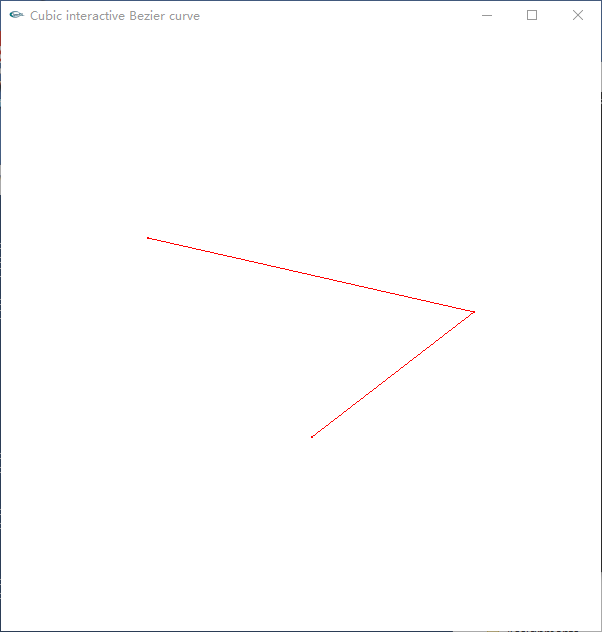
\includegraphics[width=0.5\linewidth]{fig/res1.png}&
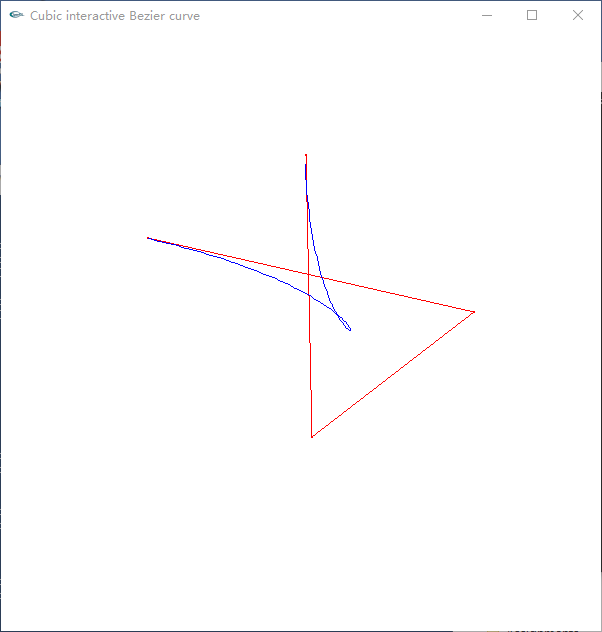
\includegraphics[width=0.5\linewidth]{fig/res2.png}
\end{tabular}
\end{figure}

\appendixconfig
\appendix
\section{源代码}
\begin{lstlisting}
#include <windows.h> // must be the first one to be included!
#include <GL/glut.h>
#include <math.h>
#include <stdio.h>

#define WIN_WIDTH 600
#define WIN_HEIGHT 600

class Point
{
public:
    Point() : x(0), y(0) {}
    Point(int px, int py) {
        set(px,py);
    }
    void set(int px, int py) {
        this->x = px;
        this->y = py;
    }
    int x, y;
};

static int num_points = 0;
static Point points[4];

void init(void)
{
    glClearColor(1.0, 1.0, 1.0, 0); // set bg color -> black
    glColor3f(0.0,0.0,0.0); // drawing color -> white
    glPointSize(2.0);
    // be careful: need to set projection!
    glMatrixMode(GL_PROJECTION);
    glLoadIdentity();
    glOrtho(0.0,WIN_WIDTH,0.0,WIN_HEIGHT,1,-1);
}

void drawPoint(Point p) {
    glBegin(GL_POINTS);
    glVertex2f(p.x, p.y);
    glEnd();
    glFlush();
}

void drawLine(Point p1, Point p2) {
    glBegin(GL_LINES);
    glVertex2f(p1.x,p1.y);
    glVertex2f(p2.x,p2.y);
    glEnd();
    glFlush();
}

Point drawBezier(Point p1, Point p2, Point p3, Point p4, double t) {
    // B(t) = P_0 (1-t)^3 + 3P_1 t(1-t)^2 + 3P_2 t^2(1-t) + P_3 t^3, t\in[0,1]
    double a1 = pow((1 - t), 3);
    double a2 = 3 * t * pow((1 - t), 2);
    double a3 = 3 * pow(t, 2) * (1 - t);
    double a4 = pow(t, 3);
    Point p(a1*p1.x + a2*p2.x + a3*p3.x + a4*p4.x,
            a1*p1.y + a2*p2.y + a3*p3.y + a4*p4.y);
    return p;
}

void myDisplay()
{
    glClear(GL_COLOR_BUFFER_BIT);
    glFlush();
}

void mouseKicked(int button, int state, int x, int y) {
    if (state == GLUT_DOWN)
    {
        // be careful that y increases from top to bottom
        points[num_points].set(x,WIN_HEIGHT-y);

        // draw point
        glColor3f(1.0,0.0,0.0); // red
        if (num_points == 0) // clear the previous curve
            myDisplay();
        drawPoint(points[num_points]);

        // draw line
        glColor3f(1.0,0.0,0.0); // red
        if (num_points > 0)
            drawLine(points[num_points-1], points[num_points]);

        // update num_points
        if (num_points == 3) {

            glColor3f(0.0,0.0,1.0); // blue

            // draw curve in small segements
            Point p_curr = points[0];
            for (double t = 0.0; t <= 1.0; t += 0.01)
            {
                Point p_new = drawBezier(points[0], points[1], points[2], points[3], t);
                drawLine(p_curr, p_new);
                p_curr = p_new;
            }

            num_points = 0;
        } else {
            num_points++;
        }
    }
}

int main(int argc, char *argv[])
{
    glutInit(&argc, argv);
    glutInitDisplayMode(GLUT_RGB | GLUT_SINGLE);
    glutInitWindowPosition(100, 100);
    glutInitWindowSize(WIN_WIDTH, WIN_HEIGHT);
    glutCreateWindow("Cubic interactive Bezier curve");
    printf("Please click left button of mouse to input control point of Bezier curve!\n");

    init();
    glutMouseFunc(mouseKicked);
    glutDisplayFunc(myDisplay); 
    glutMainLoop();
    return 0;
}
\end{lstlisting}
编译指令如下:
\begin{flushleft}
\verb'g++ bezier.cpp -I.\include -L.\lib -lglut32 -lopengl32 -o bezier.exe'
\end{flushleft}

\end{document}

% 题目:用 OpenGL 实现交互式三次 Bezier 曲线的构建,如图 1。
% 功能要求: 1. 使用鼠标在程序窗口内任意选取 4 个控制顶点;
% 2. 根据选定的控制顶点,绘制出对应的三次 Bezier 曲线,以及其控制多边形;
% 3. 语言不限,开发平台不限。具体效果展示允许略有差异。
% 实现提示: 1. 使用鼠标回调函数,捕获屏幕窗口内点的坐标。
% 要求: 1. 作业按百分制评分,没交作业算 0 分; 2. 提交代码文件,缺源代码文件的作业成绩减 10 分; 3. 提交直接可执行的程序文件或脚本文件,不能运行的程序(含出错,缺 dll 文件等)作业成绩减 10 分; 4. 作业文档,包含简要的程序文件说明,运行方法,以及程序运行结果截图,缺文档的作业成绩减 10 分; 5. 发现作业抄袭的本次作业算 0 分。
% DDL 10.30